\documentclass[../../lecture_notes.tex]{subfiles}

\begin{document}

\noindent We have worked with object-oriented languages before, \\
\indent BUT there is a difference between OO-Languages and OO-Programming.\\
We can write object-oriented programs in C (or even assembly)\\
	\indent We would use ‘struct’ for classes.\\
	\indent We would use a table of pointers to functions for virtual functions.\\
	\indent …\\
BUT we can also write non object-oriented programs using OCaml.\\

But even object-oriented programming itself is not a monolith:\\
Consider the implementation of Python and that of Java:
	\begin{itemize} [itemsep=0mm]
		\item Python uses dynamic typing whereas Java uses static.\\
			Thus Java has a more complicated syntax (interfaces. abstract classes, generics)
		\item Many properties, however, are shared:
			\begin{itemize} [itemsep=0mm]
				\item Classes bundle together fields and functions.
				\item Instantiation is the way to create objects.
				\item Inheritance is class-based.
				\item Classes are types.
				\item Classes control namespaces
			\end{itemize}
	\end{itemize}

One area of large variance is in the version of inheritance that the language uses:
\indent Java uses single inheritance — classes form a tree rooted at ‘Object’.
	\begin{lstlisting} [language=Java]
		o.m(); 
		// look in o's class, 
		// then its parent, 
		// grandparent, ad in infinitum
	\end{lstlisting}
\indent  Python uses multiple inheritance — classes form a DAG, and rules are more complicated.
	\begin{lstlisting} [language=Python]
		o.m()
		# look in o's class, 
		# up each of its parents' ancestry trees, 
		# sequentially
	\end{lstlisting}
So is Java object oriented? some people say no, since it has primitives.\\
Is Scheme object oriented? in some ways, since all data is treated as an object.\\
We can thus see that we need to be careful when others say ‘object oriented’.\\
\\
\noindent Javascript, however, takes a different approach to object-oriented programming:\\
\indent This approach is called prototype-based (as opposed to class-based).\\
\indent In Java, there are two main ways to create an object of type T.
	\begin{lstlisting} [language=Java]
		T x = new T();
		// OR
		T o = ...;
		T x = o.clone();
	\end{lstlisting}
	\indent \indent Javascript only allows instantiation via the 'clone' method.
	\begin{lstlisting} [language=Java]
		Thread t;
		// clone a class ("prototype")
		greenthread = t.clone();
		// modify it to be how you like
		greenthread.color = "green";
		// we then treat greenthread as a prototype in itself
		gt = greenthread.clone();
	\end{lstlisting}
	\indent Thus inheritance is left to us, which gives us more control and simplifies at the low level.\\
There has been a lot of ink spilled debating prototype vs class-based oo-programming.\\
\indent Prototyping tends to work well with dynamic type checking.\\
\indent The class-based approach works well with static type checking.\\
\\
Another area with multiple approaches is the method of parameter passing a language uses.\\
This, as well as syntax comes down to the issue of correspondence;\\
 How do we match the caller’s arguments with the callee’s parameters?
\begin{enumerate} [itemsep=0mm]
	\item Positional Correspondence $\equiv$ match based on position in the parameter list.\\
 		This is an approach taken by C, LISP, and most languages since FORTRAN
	\item Varargs Correspondence $\equiv$ match a fix number of parameters, then pool the rest.\\
		This can be seen in Scheme:
		\begin{lstlisting} [language=Lisp]
		(define foo (lambda (x . rest) ...))
		(foo 1 2 3 4) ; -> {x/1, rest/(2, 3, 4)}
		\end{lstlisting}
		Python takes a similar approach:
		\begin{lstlisting} [language=Python]
		def foo(x, *rest):
		  ...
		foo(1, 2, 3, 4) # -> {x/1, rest/[2, 3, 4]}
		\end{lstlisting}
 	\item Keyword/Key Correspondence $\equiv$ the caller specifies the argument/parameter binding.\\
		Python allows this:
		\begin{lstlisting} [language=Python]
		def arctan(y, x):
		  ...
		arctan(x=5, y=10)
		\end{lstlisting}
		Python even allows mixing of the three
		\begin{lstlisting} [language=Python]
		def f(x, *y, **z):
		  ...
		f(1, 2, 3, x=10, y=20 
		# -> {x/1, y/(2, 3), z/{'x'=10, 'y'=20}}
		\end{lstlisting} \smallskip
\end{enumerate}
\noindent Semantics come down to the issue of calling conventions.\\
These are more important to programmers since they affect correctness.\\
There are many methods of calling functions:
\begin{enumerate} [itemsep=0mm]
	\item \textbf{\underline{call by value}}\\
		$\equiv$ caller evaluates arguments, gets values, and passes to callee;\\
				callee then has a copy and can do whatever it wants with it
		\begin{lstlisting} [language=C]
		// caller:
		y = f(x);
		assert(y == x);
		// callee:
		x++;
 		return x;
		\end{lstlisting}
 		This can cause performance problems:
		\begin{enumerate} [itemsep=0mm]
			\item Suppose a large value space (ie a long array)
			\item Suppose an expensive function call
			\item Suppose an unused result or error — extra computation!
		\end{enumerate}
	\item \textbf{\underline{call by reference}}\\
		$\equiv$ caller passes a copy of a pointer that the callee can inspect/verify\\
		This is commonly used in C:
		\begin{lstlisting} [language=C]
	int f(int &x) {return x++;}
	z = 9;
	return f(z);
	// in C, this is compiled as if it were
	int f(int *px) { return (*p)++; }
	int z = 9;
	return f(&z);
		\end{lstlisting}
		This avoids copying overhead, but introduces problems with aliasing:
		\begin{lstlisting} [language=C]
	void trouble(int &x, int &y) {
	  x = 5;
	  y = x + 7;
	}
	int z = x;
	trouble(&x, &z); // TROUBLE
	void trouble (int &x, int &y) {
	  x = 5;
	  y = x + 7;
	  z = x; // x has gotta be 5 here, normally
 	} //  (BUT NOT ALWAYS); consider:
	z = x = 5; 
	y = 12; 
	// Faster and equivalent, right?
	// Nope, not if you have call by reference.
	//
	// aliasing introduces complications:
	int n = 10;
	int z;
	trouble (n, n); 
	// compiler cannot optimize because aliasing is possible
	\end{lstlisting}
	There are, however, ways to get around these optimization limits
	\begin{lstlisting} [language=C]
	char *strcpy(char restrict *dist, char const restrict *src);
	strcpy(x, x); // GCC compiler warning -- no aliasing
		\end{lstlisting}
	\item \textbf{\underline{call by result}}\\
		$\equiv$ caller tells callee where the result should go, and the result is copied there//
		This lets a function return a varying result.\\
		This lets functions communicate in the opposite direction as call by value.\\
		The variable is instantiated on call and initialized on return.\\
		This is commonly used in ‘Ada’, but is used in C as well:
		\begin{lstlisting} [language=C]
	<unistd.h>
	  ssize_t read(int filedes, void *buf, size_t nbyte);
	  // buf is really a call by result!
		\end{lstlisting}
	\item \textbf{\underline{call by unification}}\\
		$\equiv$ parameters are unified by compiler.\\
		This is the approach of Prolog.
	\item \textbf{\underline{call by value-result}}\\
		$\equiv$ parameter is passed by value and returned by result.\\
		The callee thus has a copy it can modify which isn’t changed until return.
		\begin{lstlisting} [language=C]
		int x = 5;
		int f(int n) {n++; return n + x;}
		f(x); // copy n in and copy result to n
		\end{lstlisting}
	\item \textbf{\underline{call by macro expansion}}\\
		$\equiv$arguments are a built in piece of the program, and so is the result.\\
		Utilized by Scheme, C/C++, etc
	\item \textbf{\underline{call by name}}\\
		$\equiv$ caller does not evaluate arguments, but instead tells the callee how to evaluate.\\
		The callee can then choose to utilize the description whenever it likes.\\
		This treats each parameter like an anonymous function.\\
		Call by name is to atoms as call by referral is to pointers.\\
		This can be done in C++++:
		\begin{lstlisting} [language=C++]
	int f(int (*xf) (void)) {return (*xf)() + 3;}
	// this is compiled like:
	int z = 9;
	int zhelp(void) {return z;} // this is a 'thunk'
	return f(zhelp);
	// This gives us a way to wait to evaluate!
	void print_avg(int arg, int n) {
	  if (n == 0) print(****);
	  else print("\%d iters, avg is \%d\n", n, avg);
	}
	print_avg(100/0, 0); 
	// this succeeds with call by name because of lazy evaluation
	// this succeeds with call by value because of eager evaluation
		\end{lstlisting}
		Our programs thus just set up a computation to be done later (often via thunks).\\
		Nothing happens until output is needed.\\
		This can be extended to \textbf{\underline{call by need }}.\\
		$\equiv$ call by name + cache results of thunks (Haskell, etc.).\\
		The ‘anonymous functions’ returned for parameters need only be run once.\\
		It’s easy to say let x = (list of all prime numbers).\\
		It’s easy to compute with infinite objects.\\
\end{enumerate} \smallskip

The syntax we have been focusing on all quarter tends to be the easier part of language.\\
Semantics tend to be much harder, and is broken into two categories:
\begin{enumerate} [itemsep=0mm]
	\item \textbf{\underline{static semantics}} $\equiv$ meaning you can tease out before the program runs
	\item \textbf{\underline{dynamic semantics}} $\equiv$ meaning that won’t be known until the program is run
\end{enumerate}
\noindent Among semantics, static is considered easy, and dynamic hard
\\
We can deal with each of these elements with the following tools:
\begin{itemize} [itemsep=0mm]
	\item syntax — BNF, EBNF, syntax charts, etc
	\item static semantics — attribute grammars
		Each node in the BNF parse tree has extra information, called “attributes”.
		These say something about the running of the program beyond the BNF.
\end{itemize}

\begin{wrapfigure}{r}{0.2\textwidth}
	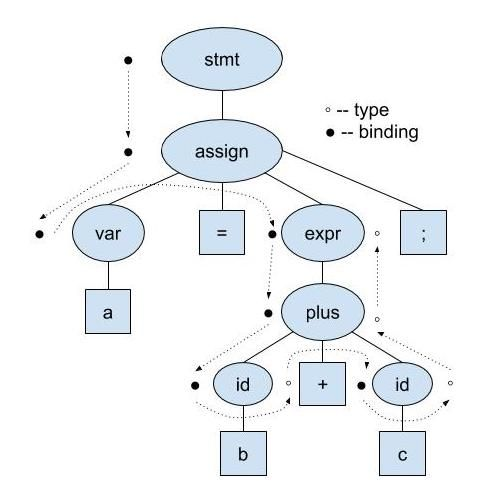
\includegraphics[width=0.2\textwidth]{attribute_tree}
	\label{fig:test}
\end{wrapfigure}

Consider the expression ‘a = b + c’;\\
\indent This can form the tree (right).\\
Downward inference is called \textbf{\underline{inheritance}}.\\
Upward inference is called \textbf{\underline{synthesis}}.\\
These let us derive information from grammar rules\\
\indent plus $\rightarrow$ id + id\\
\indent \indent type(plus) = \\
\indent \indent \indent if type(id1) == type(id2) == int\\
\indent \indent \indent \ \ then int\\
\indent \indent \indent \ \ else float\\
\indent expr → plus\\
 \indent \indent type(expr) = type(plus)\\
\\ 
 Dynamic semantics must further be broken into three broad categories:
 \begin{enumerate} [itemsep=0mm]
	\item \textbf{\underline{operational}}\\
		$\equiv$ describe writing an interpreter — derived from imperative languages.\\
		For example, Python is defined by an interpreter, C-Python, written in C.
	\item \textbf{\underline{axiomatic}}\\
		$\equiv$ logic you can use to reason the program — derived from logic languages.\\
		For example, the first semantics for lisp were defined in Lisp.\\
		This is philosophically “bad” but interesting in practice, like an English dictionary
	\item \textbf{\underline{denotational}}\\
		$\equiv$ function: program → meaning — derived from functional languagea.
\end{enumerate}
\noindent This is simplified of course.
\\
Allow us to attempt to use method (c) to define a subset of OCaml in Prolog:\\
\begin{lstlisting} [language=Prolog]
		m(E1+E2, C, Vsum) :-
		  m(E1, C, V1),
		  m(E2, C, V2),
		Vsum is V1 + V2).
		% we have thus defined a high level '+' by a lower level '+'
		m(K, C, K) :- integer(K).
		% defines constants
		m(Var, C, Val) :- member(Var=Val, C).
		% defines variable binding
		m(let(X, E1, E2), C, Val) :-
		  m(E1, C, V1),
		  m(E2, [X=V1|C], Val).
		% defines 'let' binding
		m(fun(X, E), C, lambda(X, E)).
		% functions need not be evaluated
		m(call(E1, E2), C, Result) :-
		  m(E1, C, lambda(Xf, Ef)),
		  m(E2, C, V2),
		  m(Ef, [Xf=V2|C], Result).
\end{lstlisting}
\noindent These semantics use dynamic scoping; static would be more complicated.\\
\\
The history of programming languages in a few lines, according to Paul Eggert:\\
	\indent “Lots of attempts to ‘take over the world’”\\
	\indent “None have succeeded”\\
	\indent “We still have a lot of variety, and that is not going away”\\
	Thus we must keep always the basic principals in mind

\end{document}